\documentclass[12pt]{article}
\usepackage[margin=1in]{geometry}
\usepackage{graphicx}
\usepackage{booktabs}
\usepackage{longtable}
\usepackage{hyperref}
\usepackage{natbib}
\title{A Closed-Water-Balance Ecohydrological Model Benchmark for 671 CAMELS Basins Across the Conterminous United States}
\author{Author placeholders}
\date{}
\begin{document}
\maketitle
\section*{Key Points}
\begin{itemize}
\item The closed Model 6 benchmark achieves strong continental streamflow skill while preserving near-exact water-balance closure.
\item Independent FLUXCOM and MOD16 ET diagnostics support broad ET realism, but local GLEAM products were unavailable for this build.
\item JPL GRACE supports moderate large-scale storage realism, while small-basin storage comparisons remain exploratory.
\end{itemize}
\begin{abstract}
The closed Model 6 benchmark achieved median NSE 0.685 and median KGE 0.643 with a median absolute daily closure residual of 0.000183 mm/day.
\end{abstract}
\section*{Plain Language Summary}
We assembled a reproducible continental hydrology benchmark package and evaluated it with independent evapotranspiration and storage products.
\section{Introduction}
Large-sample hydrologic models need both predictive skill and physically credible internal organization.
\section{Methods}
The authoritative run is `Model6Closed_Snow_aSrz_SIMHYD_Simple_full671_ep100_iter200`. State-rich daily diagnostics use the existing Ep60 auxiliary archive when no Ep100 state export was available locally.
\section{Results}
Median streamflow NSE was 0.685; median KGE was 0.643. Median FLUXCOM ET NSE was 0.468 across 164 basins. Median JPL GRACE basin NSE was 0.351.
\begin{figure}[ht]
\centering
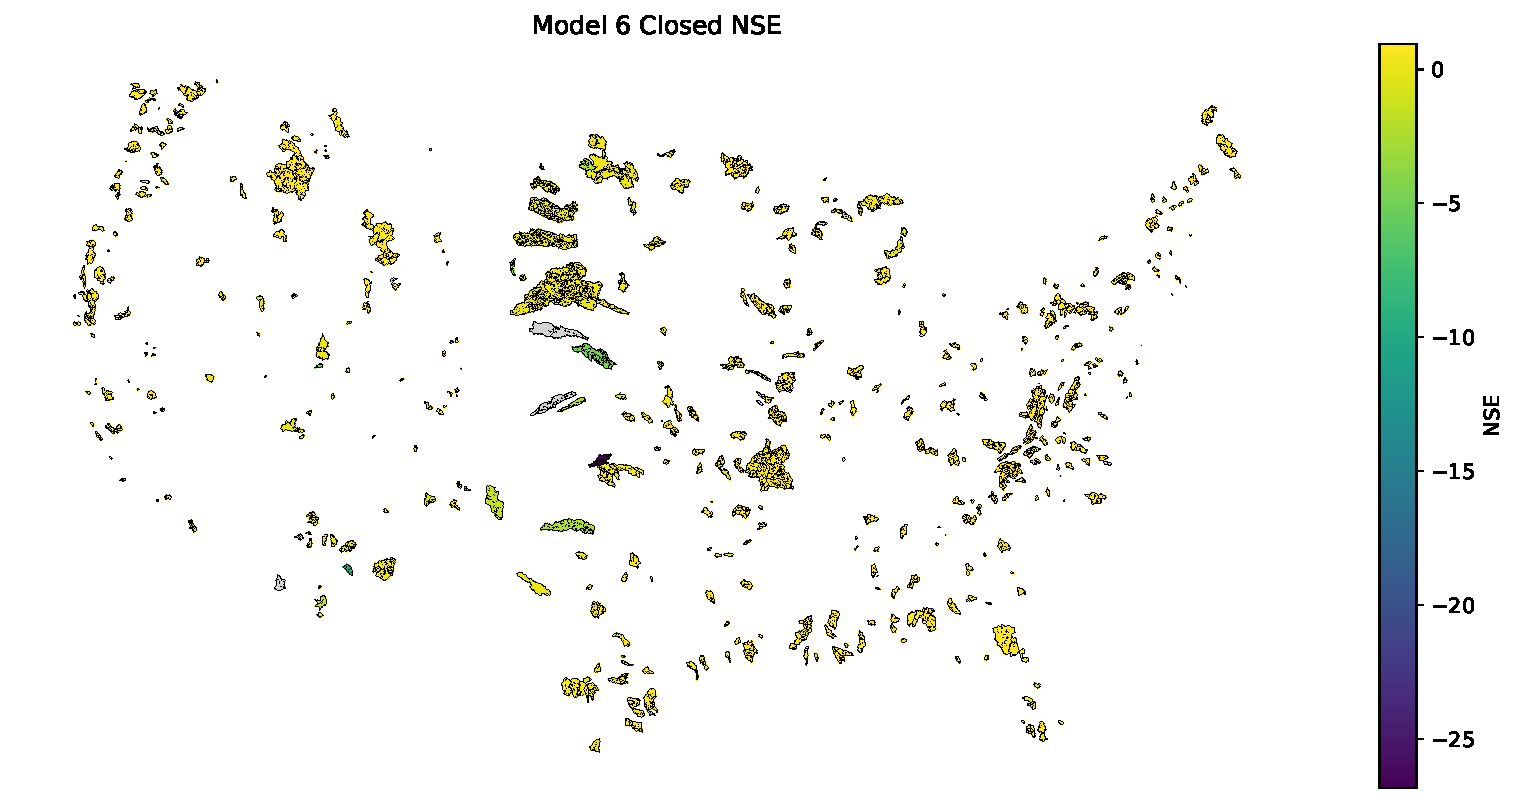
\includegraphics[width=\textwidth]{figures/map_NSE.pdf}
\caption{Spatial distribution of streamflow prediction skill across the 671 CAMELS basins. NSE values are shown on a fixed 0--1 scale to emphasize differences among basins with non-negative skill. Values below 0 are clipped to 0 for visualization only; original values are retained in the basin-level metric table.}
\end{figure}
\begin{figure}[ht]
\centering
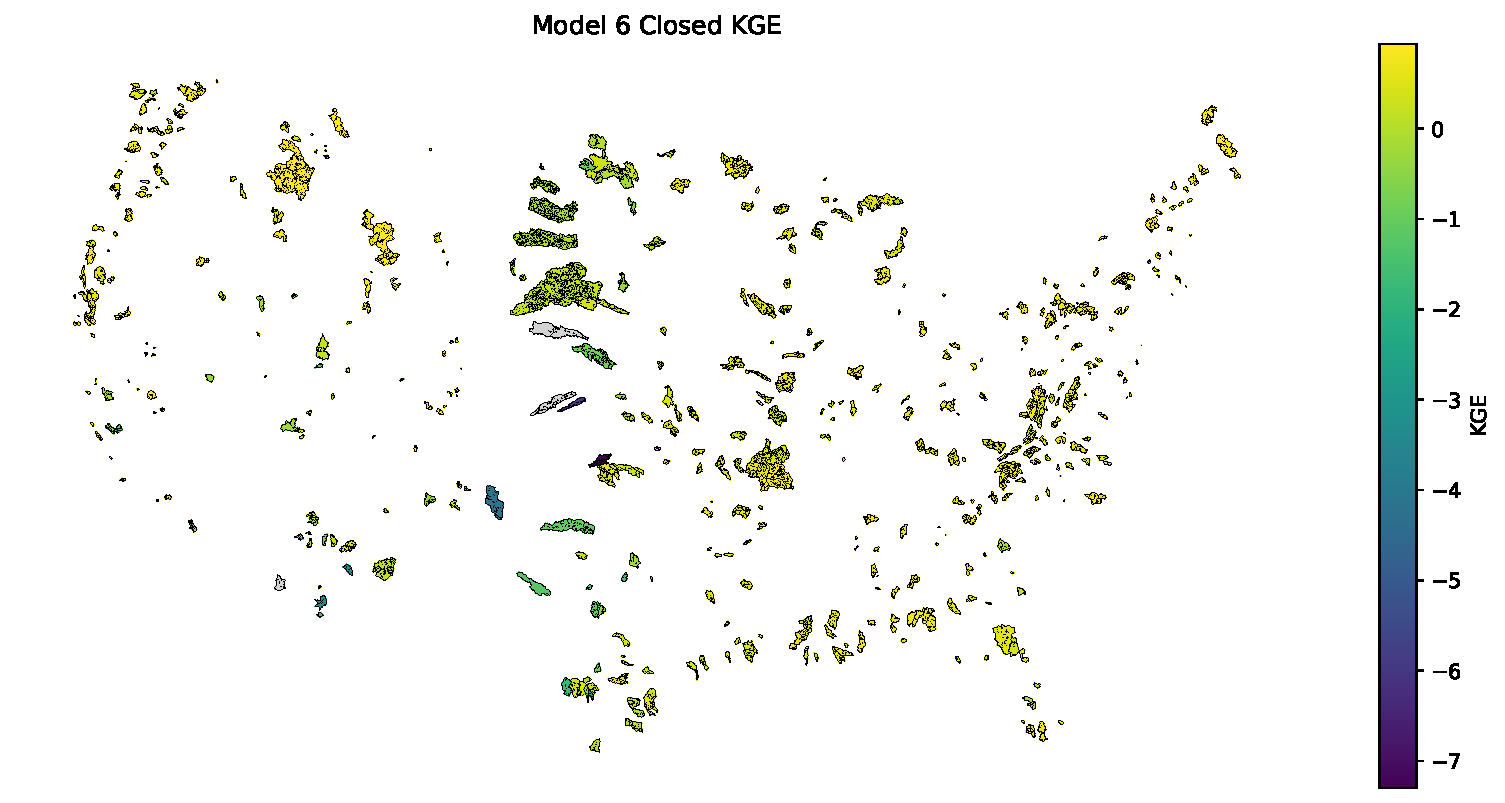
\includegraphics[width=\textwidth]{figures/map_KGE.pdf}
\caption{Spatial distribution of Kling-Gupta efficiency across the 671 CAMELS basins. KGE values are shown on a fixed 0--1 scale for visual comparability. Values below 0 are clipped to 0 for visualization only; original values are retained in the basin-level metric table.}
\end{figure}
\begin{figure}[ht]
\centering
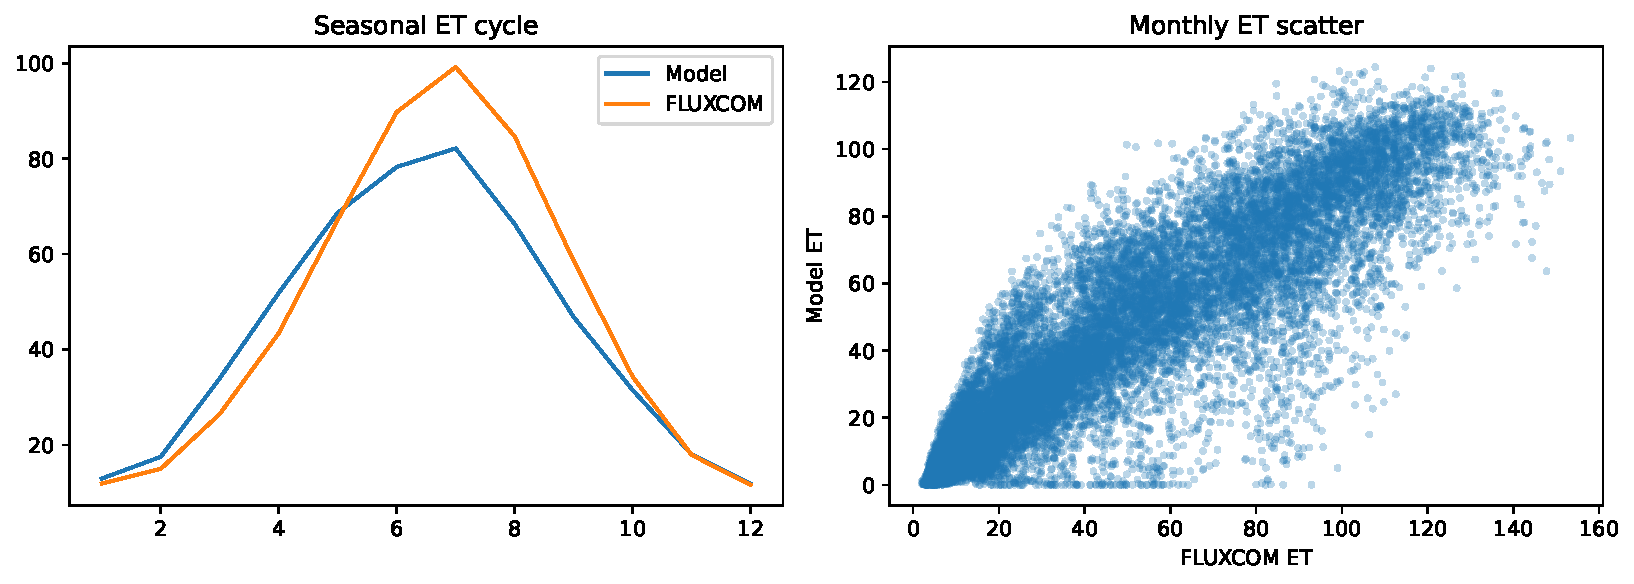
\includegraphics[width=\textwidth]{figures/et_validation_summary.pdf}
\caption{Monthly and seasonal evapotranspiration validation against FLUXCOM with MOD16 used as an annual cross-check.}
\end{figure}
\begin{figure}[ht]
\centering
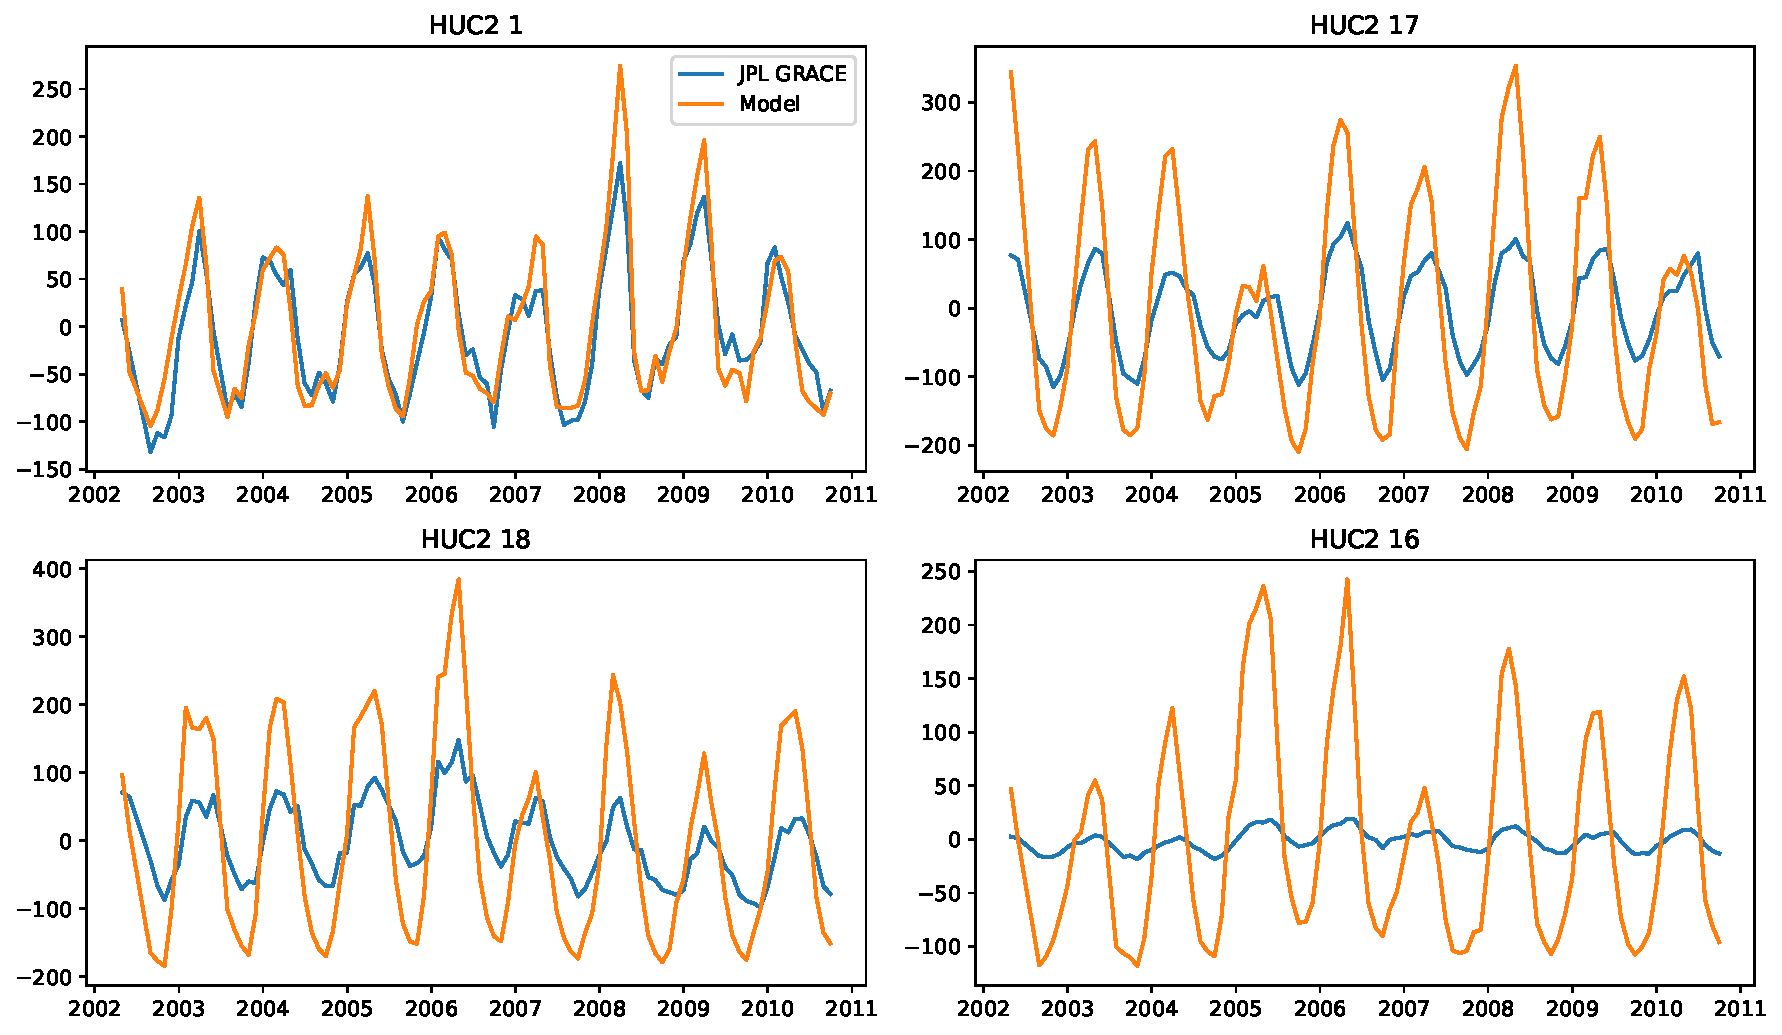
\includegraphics[width=\textwidth]{figures/twsa_regional_timeseries.pdf}
\caption{Regional comparison between model TWSA and JPL GRACE TWSA.}
\end{figure}
\section{Discussion}
The model should be interpreted as a closure-preserving diagnostic benchmark rather than a claim of fully constrained internal realism.
\section{Conclusions}
The benchmark supports a model-development and evaluation paper with explicit caveats about ET product disagreement, GRACE scale mismatch, and inferred storage capacity.
\section*{Data Availability}
All generated outputs are organized under `WRR_Model6_EndToEnd_Paper/`.
\section*{Code Availability}
All scripts used to generate the package are stored under `WRR_Model6_EndToEnd_Paper/scripts/`.
\section*{Acknowledgments}
Acknowledgments placeholder.
\bibliographystyle{plainnat}
\bibliography{references}
\end{document}
